\section[The Riemann-Stieltjes Integral]{\hyperlink{toc}{The Riemann-Stieltjes Integral}}

\subsection{Definition of the Integral}
\begin{definition}{Partition}{6.1}
    A partition of $[a, b] \subset \RR$ is a set $\set{x_0, x_1, \ldots, x_n}$ (for some $n \in \NN$) such that:
    \begin{align*}
        a = x_0 \leq x_1 \leq x_2 \leq \ldots \leq x_{n-1} \leq x_n = b
    \end{align*}
    We can then write:
    \begin{align*}
        \Delta x_i = x_i - x_{i-1} 
    \end{align*}
\end{definition}

\begin{figure}[htbp]
    \centering
    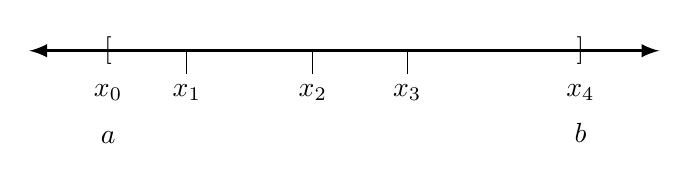
\begin{tikzpicture}[scale=2]
        \draw[very thick, latex-latex] (-2, 0) -- (2, 0);
        \node[] at (-1.5, 0) {$[$};
        \node[below] at (-1.5, -0.15) {$x_0$};
        \node[below] at (-1.5, -0.45) {$a$};
        \node[] at (1.5, 0) {$]$};
        \node[below] at (1.5, -0.15) {$x_4$};
        \node[below] at (1.5, -0.4) {$b$};
        \draw[] (-1, 0) -- (-1, -0.15);
        \node[below] at (-1, -0.15) {$x_1$};
        \draw[] (-0.2, 0) -- (-0.2, -0.15);
        \node[below] at (-0.2, -0.15) {$x_2$};
        \draw[] (0.4, 0) -- (0.4, -0.15);
        \node[below] at (0.4, -0.15) {$x_3$};
    \end{tikzpicture}
    \caption{Visualization of a partition $\set{x_0, x_1, x_2, x_3, x_4}$ of $[a, b]$. Note that the points in the partitions need not be equally spaced.}
    \label{fig27}
\end{figure}

\setcounter{rudin}{0}
\begin{definition}{Upper and Lower Sums}{6.1}
    Given $f: [a, b] \mapsto \RR$ and a partition $P$ of $[a, b]$ let:
    \begin{align*}
        M_i &= \sup\set{f(x): x_{i-1} \leq x \leq x_i}
        \\ m_i &= \inf\set{f(x): x_{i-1} \leq x \leq x_i}
    \end{align*}
    Then, we can define the upper and lower sums:
    \begin{align*}
        U(P, f) &= \sum_{i=1}^n M_i \Delta x_i
        \\ L(P, f) &= \sum_{i=1}^n m_i \Delta x_i
    \end{align*}
\end{definition}

\begin{figure}[htbp]
    \centering
    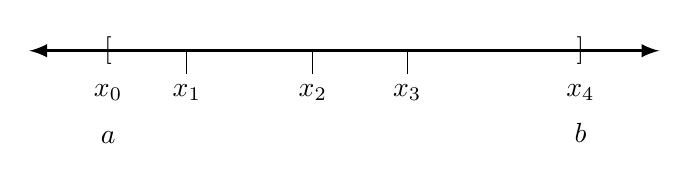
\begin{tikzpicture}[scale=2]
        \draw[very thick, latex-latex] (-2, 0) -- (2, 0);
        \node[] at (-1.5, 0) {$[$};
        \node[below] at (-1.5, -0.15) {$x_0$};
        \node[below] at (-1.5, -0.45) {$a$};
        \node[] at (1.5, 0) {$]$};
        \node[below] at (1.5, -0.15) {$x_4$};
        \node[below] at (1.5, -0.4) {$b$};
        \draw[] (-1, 0) -- (-1, -0.15);
        \node[below] at (-1, -0.15) {$x_1$};
        \draw[] (-0.2, 0) -- (-0.2, -0.15);
        \node[below] at (-0.2, -0.15) {$x_2$};
        \draw[] (0.4, 0) -- (0.4, -0.15);
        \node[below] at (0.4, -0.15) {$x_3$};
    \end{tikzpicture}
    \caption{Example of a function $f$, a partition $P$ of $[a, b]$, and the $M_i, m_i$s for this choice of partition.}
    \label{fig28}
\end{figure}

\noindent By construction, it should be evident that $L(P, f) \leq U(P, f)$ for all $P, f$.

A natural question that arises from the form of the above expression is whether these are Riemann sums or not. Recall from first year calculus that we would choose the left endpoint, right endpoint, or some other arbitrary choice of a point in the subinterval. Here, we in a sense use a ``special case'' of the supremum/infimum. We will see that this choice is musch easier to use in proofs due to monotonicity properties. Namely, if we have a partition and add another point, then $U(P, f)$ can only decrease, and $L(P, f)$ can only increase (we will see this in a theorem soon)!


\setcounter{rudin}{0}
\begin{definition}{Upper/Lower Integrals and Riemann Integrability}{6.1}
    We define the Upper Riemann Integral to be:
    \begin{align*}
        \uint{a}{b} = \inf_P U(P, f).
    \end{align*}
    and the Lower Riemann Integral to be:
    \begin{align*}
        \lint{a}{b} = \sup_P L(P, f).
    \end{align*}
    Here, the infimum/supremum is taken over all partitions $P$. We say that $f$ is Riemann integral in
\end{definition}

\subsection{Criterion for Integrability}

\subsection{Properties of the Integral}

\subsection{Integration and Differentiation}

